\documentclass[10pt,english]{article}
\usepackage{geometry}
\geometry{
a4paper, 
lmargin=1.5cm,
rmargin=1.5cm,
tmargin=2cm,
bmargin=3cm
}
\usepackage[utf8]{inputenx}
\usepackage{babel}
\usepackage[T1]{fontenc}
\usepackage{graphicx}
\usepackage{paralist}
\usepackage[parfill]{parskip}
\usepackage{mathtools}
\usepackage{amssymb}
\usepackage{physics}
\usepackage{float}
\usepackage{xstring}
\usepackage{url}
\usepackage{siunitx}
\usepackage{xspace}
\usepackage{subcaption}
\usepackage[font=small,labelfont=bf]{caption}
\usepackage{wrapfig}

\mathtoolsset{showonlyrefs=true}

\title{Project TMA4220: Finite Element Method}
\author{XXX, YYY}
\date{}

\begin{document}
\maketitle

%% !TEX root = ../main/main.tex
\begin{abstract}
bla bla bla
\end{abstract}
% !TEX root = ../main/main.tex
\section{Introduction}
Heat sinks are a commonly used heat exchangers with the purpose of transferring heat that are generated by electronic or mechanical devices \cite{wiki_hs}. In computers it is useful to be able to regulate the temperature of components like the central processing unit (CPU) or the graphic processing unit	(GPU). These units typically generate a lot of heat and it becomes necessary for optimal operation to dissipate this heat away to keep the temperature at an optimal level. This is typically done by using a heat sink together with a fan as seen in \cref{fig:heatsink_and_fan}. 

\begin{wrapfigure}{r}{0.5\textwidth}
	\begin{center}
		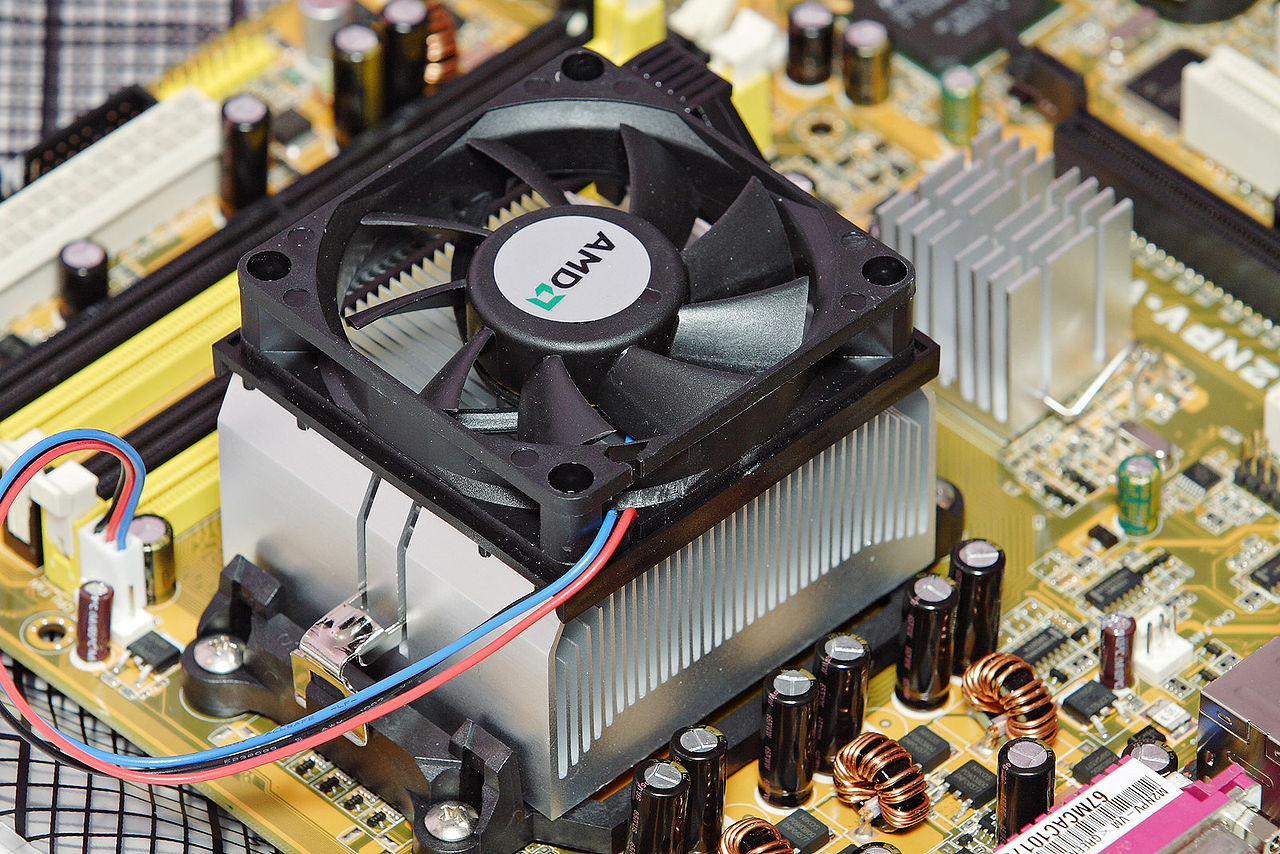
\includegraphics[width=0.48\textwidth]{../figures/heatsink_and_fan.jpg}
	\end{center}
	\caption{Heat sink and fan on processing unit. Source: \cite{wiki_hs}}
    \label{fig:heatsink_and_fan}
\end{wrapfigure}

When designing heat sinks one typically tries to maximize surface area in contact with the cooling medium surrounding it, such as air. There are several factors that affects the performance of a heat sink. In essence air velocity, choice of material, design and surface treatment are the most important ones. When choosing material one should look for good heat conductors which means that heat can be transferred though the material quickly. In many cases copper is used because of its excellent thermal efficiency.

In this report we will be trying to use a Finite Element Method to evaluate the effect of increasing the surface area on a simple heat sink design in two different ways. One ways is to extend the length of the fins, and the other is to increase the number of fins. We will keep the geometric properties of the heat sink base constant, meaning that we will only vary the geometry of the fins themselves. This report is divided into three main parts. In the \textit{Theory} part we will elaborate on the heat equation and show a finite element analysis which results in a linear system of equations. In the \textit{Numerical Implementations} part we will go through and explain the steps of implementing the numerical interpretation. In the \textit{Results and Discussion} we will present our results together with a discussion of their interpretation. Finally we will conclude our findings and suggest improvements for further work. %TODO: Check the correct section names.

% !TEX root = ../main/main.tex
\section{Theory}
\subsection{The problem}
The heat equation of a material with thermal conductivity $k$ is given as
\begin{equation}
	k\laplacian{u(\vb{x},t)} = \pdv{u(\vb{x},t)}{t}
	\label{eq:gen_heat_eq},
\end{equation}
with the Dirichlet condition $u(\vb{x},t) = g(\vb{x},t)$ on the boundary, for some given function $g$. If we insetad look at the stationary case, the right hand side of \eqref{eq:gen_heat_eq} becomes zero. In addition if instead of looking at the inhomogenous Dirichlet boundary condition.

Let $\Omega \subset \mathbb{R}^n$ be bounded, open set, and let $u(\vb{x})$ satisfy the boundary value problem 

\begin{alignat}{3}
	\laplacian{u(\vb{x})} &= 0 &&,\quad u(\vb{x}) \in \Omega \\
	u(\vb{x}) &= u_0 &&,\quad u(\vb{x}) \in \partial\Omega_D \\
	k\pdv{u(\vb{x})}{n} &= -h\left(u(\vb{x}) - u_{amb} \right) &&, \quad u(\vb{x}) \in \partial\Omega_R.
	\label{eq:heat_bvp}
\end{alignat}
Here the temperature $u_0$ and the ambient temperature $u_{amb}$ are fixed, while $h$ is the heat transfer coefficient between two materials. $\partial\Omega_D$ and $\partial\Omega_R$ denotes the Dirichlet and Robin part of the boundary $\partial\Omega = \partial\Omega_D\cup\Omega_R$, respectively. In the Robin boundary condition  $\vb{n}$ is the outward normal unit vector. The term $\pdv*{u}{n}$ is the heat flux, and is in this model proportional to the temperature difference between the ambient temperature and the solution. The minus sign emphasizes that the heat is flowing in the opposite direction of the temperature gradient, which is reasonable.

\subsection{Weak form}
The finite element method requires the PDE to to be formulated in terms of its weak form. We introduce a set of test functions $C_0^\infty(\Omega)$. This is the set of all infinitely differentiable functions with compact support in $\Omega$. $V = H_0^1(\Omega)$ is the Sobolov space. By Green's formula we have
\begin{equation}
	\int_\Omega \! v\laplacian{u} \, \mathrm{d}\Omega = \int_{\partial\Omega} \! v\pdv{u}{n} \, \mathrm{d}\gamma -  \int_\Omega \! \grad{u}\cdot\grad{v} \, \mathrm{d}\Omega = 0
	\label{eq:green}.
\end{equation}
The boundary integral is split up into the $\partial\Omega_D$ and $\partial\Omega_R$. Now if $v \in V$, the integral over $\partial\Omega_D$ vanishes, and after we rearrange the terms the equation reduces to 
\begin{equation}
	\frac{k}{h}\int_\Omega \! \grad{u}\cdot\grad{v} \, \mathrm{d}\Omega + \int_{\partial\Omega_R} \! uv\, \mathrm{d}\gamma = u_{amb}\int_{\partial\Omega_R} \! v \, \mathrm{d}\gamma.
	\label{eq:weak_form}
\end{equation}
Note that because of the inhomogeneous Dirichlet boundary conditions $u \notin V$, even though the proper weak formulation should state: Find $u \in V$ such that \eqref{eq:weak_form} is satisfied $\forall v \in V$. Formally one should explicitly introduce a lifting function $R$ such that a new function $\mathring{u} = u - R$ satisfies the homogeneous Dirichlet conditions, and formulate the weak form in terms of $\mathring{u}$. However, in our numerical scheme we will get the desired solution by setting the solution of our linear system to the known Dirichlet boundary values.

From \eqref{eq:weak_form} we see that our bilinear form $a(\cdot,\cdot)$ and linear functional $F(\cdot)$ takes the form
\begin{align}
	a(u,v) &= \frac{k}{h}\int_\Omega \! \grad{u}\cdot\grad{v} \, \mathrm{d}\Omega + \int_{\partial\Omega_R} \! uv\, \mathrm{d}\gamma \\
	F(v) &= u_{amb}\int_{\partial\Omega_R} \! v \, \mathrm{d}\gamma.
	\label{eq:bilin_form}
\end{align}
Given a set of points $\left\{\vb{x}_i\right\}_{i=1}^n$ in $\Omega$, we now define a set of nodal functions $\left\{\varphi_i(\vb{x})\right\}_{i=1}^n$, such that $\varphi_i(\vb{x}_j) = \delta_{ij}$, $i,j = 1,\dots,n$. Now we define $V_h = \operatorname{span}\left\{\varphi_i(\vb{x})\right\}_{i=1}^n$, and let $u_h(\vb{x}) = \sum_{i=1}^{n} u_i \varphi_i(\vb{x}) \in V_h$. The Galerkin problem can then be formulated as "Find $u_h \in V_h$ such that $a(u_h,v) = F(v)\, \forall v \in V_h$". Since $a(\cdot,\cdot)$ is bilinear, $F(\cdot)$ is linear and $u_h$  is a linear combination of the basis functions $\left\{\varphi_i(\vb{x})\right\}_{i=1}^n$, this problem is equivalent to the linear system %TODO: tungvindt å lese
\begin{equation}
	A\vb{u} = \vb{b}, \quad A_{ij} = a(\varphi_i,\varphi_j), \,\, b_i = F(\varphi_i)
	\label{eq:lin_sys},
\end{equation}
with $\vb{u}$ being the vector with elements corresponding to the coefficients $u_i$ of $u_h$. We note that since we have not yet enforced the Dirichlet boundary conditions, the solution is not unique, hence $A$ is not invertible in its current form.

\subsection{Barycentric coordinates and numerical integration}
We only state the formulas for evaluating integrals numerically on simplexes using barycentric quadrature points. For an in-depth cover of this topic, we refer to \cite{quarteroni}. Let $\mathcal{\hat{K}}$ be the reference simplex in $\mathbb{R}^n$ with corners $\vb{\hat{e}}_1,\dots,\vb{\hat{e}}_n$ and $\vb{0}$ and  $\mathcal{K}$ be the physical simplex with corners $\vb{p}_0,\dots,\vb{p}_n$. The integral transformation then yields 

\begin{equation}
	\int_{\mathcal{K}} \! f(\vb{x}) \, \mathrm{d}V = \int_{\mathcal{\hat{K}}} \! f(\vb{\hat{x}})\frac{1}{n!}\frac{\operatorname{Volume}(\mathcal{K})}{\operatorname{Volume}(\mathcal{\hat{K}})}\, \mathrm{d}\hat{V}.
\end{equation}
The volume of the simplex $\mathcal{K}$ is \cite{wiki_simplex}
\begin{equation}
 	\operatorname{Volume}(\mathcal{K}) = \frac{1}{n!}\left|\operatorname{det}\left(\vb{p}_1-\vb{p}_0\,\dots\,\vb{p}_n-\vb{p}_0\right)\right|.
 \end{equation} 
We also note that $\operatorname{Volume}(\mathcal{\hat{K}}) = 1/n!$. Each point in $\mathcal{K}$ can be described with a barycentric coordinate $\vb{\pmb{\lambda}} = \left(\lambda_0,\dots,\lambda_{n}\right)$, with the mapping to the physical space $\vb{x} = \lambda_0\vb{p}_0 + \dots + \lambda_n\vb{p}_n$. Given a set of $m$ barycentric quadrature points, $\vb{\pmb{\lambda}}^1,\dots,\vb{\pmb{\lambda}}^m$, and corresponding weights, $\rho_1,\dots,\rho_m$, the numerical integration formula becomes
\begin{equation}
	\int_{\mathcal{K}} \! f(\vb{x}) \, \mathrm{d}V \approx \operatorname{Volume}(\mathcal{K})\sum_{i = 1}^m \rho_m f(\lambda_0^i\vb{p}_0 +\dots + \lambda_n^i\vb{p}_n).
\end{equation}
This quadrature rule is used $\texttt{quadrature2D}$ and $\texttt{quadrature3D}$, while $\texttt{quadrature1D}$ relies on gaussian quadrature. The table of barycentric quadrature points used in the code can be found in \cite{tma4220}.
%Where $k = \SI{401}{\watt\per\meter\per\kelvin}$ is the thermal conductivity of copper, and $h \approx 10$
% !TEX root = ../main/main.tex
\section{Numerical implementation}
\subsection{Basis functions}
The choice of the type of basis functions is important when implementing the finite element method. In this project we have settled for the simplest type, namely the linear type. In higher dimensions one would usually resort to reference functions in a reference space, however for linear basis functions looking at the physical space is enough. The linear functions in $\mathbb{R}^3$ is of the form
\begin{equation}
	\varphi_i(x,y,z) = a_ix + b_iy + c_iz + d_i,
\end{equation}
where the index $i$ refers to the node. In a nodal basis we want $\varphi_i(\vb{x}_j) = \delta_{ij},\, i,j = 1,\dots,n$, and in a mesh consisting of tetrahedral elements the coefficients can be calculated per element. For instance, if $\mathcal{K}_i$ is the element being the tetrahedron given by the nodes $\{j,k,l,m\}$. Then the coefficients in $\varphi_j$ is given by the solution of the linear system
\begin{equation}
    \begin{bmatrix*}[l]
        x_j & y_j & z_j & 1 \\
        x_k & y_k & z_k & 1 \\
        x_l & y_l & z_l & 1 \\
        x_m & y_m & z_m & 1
     \end{bmatrix*}
     \begin{bmatrix*}[l]
        a_j \\
        b_j \\
        c_j \\
        d_j 
    \end{bmatrix*}
    =
    \begin{bmatrix}
        1 \\
        0 \\
        0 \\
        0 \\
    \end{bmatrix}.
    \label{eq:coeff_sys}
\end{equation}

\subsection{The numerical integrals}
$a(u,v)$ in \eqref{eq:bilin_form} contains a the gradient of the basis functions $\varphi$. However because of the linearity of the basis functions this integral will be simply be the the volume of each element, multiplied by a constant. Let $\pmb{\varphi}(\vb{x}) = \left(\varphi_1(\vb{x}),\dots,\varphi_4(\vb{x})\right)^T$ be the vector of basis function on an element $\mathcal{K}$. Then each entry in the symmetric matrix
\begin{equation}
    \pmb{J}_{\pmb{\varphi}}^{\phantom{}} \pmb{J}_{\pmb{\varphi}}^T\int_\mathcal{K} \! \mathrm{d}V
\end{equation}
represent the contribution from each combination of $\grad{\varphi_i}\cdot\grad{\varphi_j}$ on $\mathcal{K}$. Here $\pmb{J}_{\pmb{\varphi}}$ is the Jacobian of $\pmb{\varphi}$. The two remaining integrals in \eqref{eq:bilin_form} are surface integrals over the boundary of $\Omega$. We can use the function \texttt{quadrature2D} to integrate over planes in $\mathbb{R}^3$ by projecting down onto $\mathbb{R}^2$. Let $\vb{p}_1,\vb{p}_2,\vb{p}_3 \in \mathbb{R}^3$. The plane going through all three points have normal vector $\vb{n} = (\vb{p}_2-\vb{p}_1)\cross (\vb{p}_3-\vb{p}_1)$. Projecting down on the $xy$-plane then yields
\begin{equation}
    z = z(x,y)=\frac{1}{n_3}\left(\vb{n}\cdot \vb{p}_1-n_1x-n_2y\right).
\end{equation}
The differential $\mathrm{d}\gamma$ on the plane then becomes
\begin{equation}
    \mathrm{d}\gamma = \frac{\norm{\vb{n}}}{\abs{n_3}}\mathrm{d}x\mathrm{d}y.
\end{equation}
The whole boundary of the mesh consists of planes normal to the all the axes, so we would actually need project onto both the $xz$- and $yz$-plane as well for different parts of the boundary. Instead we rotate the mesh $\pi/4$ around both the $x$ and the $y$-axis, using the rotation matrix
\begin{equation}
    R_x\left(\frac{\pi}{4}\right)R_y\left(\frac{\pi}{4}\right) = \frac{1}{2}
    \begin{bmatrix}
        \sqrt{2} & 0 & 0 \\
        0 & 1 & -1 \\
        0 & 1 & 1
     \end{bmatrix}
     \begin{bmatrix}
        1 & 0 & 1 \\
        0 & \sqrt{2} & 0 \\
        -1 & 0 & 1
     \end{bmatrix},
\end{equation}
yielding no boundary surface being normal to the $xy$-plane.

When calculating the contribution from the integrals over the boundary in \eqref{eq:bilin_form} we need to know which nodes are on the boundary. It is natural to keep the list of the elements and the boundary surfaces separate, and adding the contribution from each integral in separate loops in the program. The linear basis functions $\varphi$ represents a plane in $\mathbb{R}^4$, however as each surface element is a triangle, we only have three points for the system \eqref{eq:coeff_sys}. The last point can be chosen arbitrarily, but in order to avoid problems with linear dependence in the row space of \eqref{eq:coeff_sys}, we choose $\vb{n}$, which is linearly independent of $\vb{p}_1,\vb{p}_2$ and $\vb{p}_3$ .

\subsection{The Dirichlet boundary}
 The size of the linear system \eqref{eq:lin_sys} increases with the number of nodes in the mesh, it is important to keep the number of dimensions in system to a minimum. Since the solution on the Dirichlet boundary $\partial\Omega_D$ is known by definition, these nodes need not be in the vector $\vb{u}$ in \eqref{eq:lin_sys}. Instead the contribution in each row corresponding to $u_i$, where $\vb{x}_i \notin \partial\Omega_D$, can be moved to the right-hand side of the system, reducing the dimension by the number of nodes on $\partial\Omega_D$. We refer to the code as of how this was done.

 Because of the nodal basis, the integrals in \eqref{eq:bilin_form} will be zero between all non-neighboring nodes, and as a result the matrix $A$ will be sparse. However, as the finite elements works by updating $A$ and $b$ in \eqref{eq:lin_sys} while looping over all the elements, it is not known beforehand which entries of $A$ and $b$ which will be non-zero. Using \textsc{Matlab}'s\xspace \texttt{sparse} functionality was therefore not beneficial in our case. On the contrary, we do not reject the possibility that there may be other ways to exploit the sparsity of $A$.

 A heat sink has a geometry which is generally difficult to model with a 3D mesh. The surface should be as large as possible in order to maximize contact with the surrounding air. The fins should therefore be as many and as thin as possible. Because of this, tetrahedral elements may not be optimal for the type of geometries considered in this report. For instance, Comsol \cite{comsol_mesh_types} recommends to use brick or prism elements in cases where the geometry consists of thin layers.


\subsection{Generating the mesh}
 For our purposes we did not need a complex geometry so we opted for a simple geometry for the heat sinks. To create and control the geometry as we wanted, we used the software \textit{Gmsh}. For practical reasons we chose the size of the heat sink base to be $1.05\times1.05$. For the height of the base and the thickness of the fins we chose 0.05 and 0.07. These values does not change through the experiment. What we varied was the number of fins and the height of the fins. We tried 4 and 8 fins and heights of 1.0 and 2.0.

 \begin{figure*}[h t!]
 \begin{subfigure}[t] {0.23\textwidth}
 \centering
 \includegraphics[width=0.7\textwidth]{"../figures/mesh_4_1 (new)"}
 \caption{4 fins, height: 1}
 \label{fig:mesh_4_1}
 \end{subfigure}
 ~
  \begin{subfigure}[t] {0.23\textwidth}
 \centering
 \includegraphics[width=0.7\textwidth]{"../figures/mesh_8_1 (new)"}
 \caption{8 fins, height: 1}
 \label{fig:mesh_8_1}
 \end{subfigure}
 ~
 \begin{subfigure}[t] {0.23\textwidth}
 \centering
 \includegraphics[width=0.7\textwidth]{"../figures/mesh_4_2 (new)"}
 \caption{4 fins, height: 2}
 \label{fig:mesh_4_2}
 \end{subfigure}
 ~
 \begin{subfigure}[t] {0.23\textwidth}
 \centering
 \includegraphics[width=0.7\textwidth]{"../figures/mesh_8_2 (new)"}
 \caption{8 fins, height: 2}
 \label{fig:mesh_8_2}
 \end{subfigure}
 \caption{These are the different meshes we tried}
 \label{fig:meshes}
 \end{figure*}

 \begin{figure}[h]
 \centering
 \includegraphics[width=0.3\textwidth]{"../figures/meshcut (new)"}
 \caption{A more detailed inspection of the mesh}
 \label{fig:meshcut}
 \end{figure}

 % Furthermore, in our experiment \textit{Gmsh} we checked the option to use Delaunay triangulation, and we also told \textit{Gmsh} to use 3 smoothing steps when generating the mesh. For the {Geometry Mesh Size Factor} we used 0.05. 

% !TEX root = ../main/main.tex
\section{Results and discussion}



\subsection{Visualizating the results}
Visualizing the results from simulations is important in order to understand the result. When having a function in three dimensions it is necessary to make choices of what part of the result which should be displayed. The natural way of doing this is either with iso-surfaces or cutting-planes. The geometries in \cref{fig:meshes} are somewhat symmetric, especially along the fins, which suggests that the temperature field should be more or less constant along this axis. In 3D visualizing software this is easier to see, and in our solution this is indeed the case. Therefore \cref{fig:mesh_temps} represents a cutting plane normal to the fins, which should give a good representation of the temperature field in the whole geometry.

\begin{figure}[ht]
\begin{subfigure}[t] {0.23\textwidth}
\centering
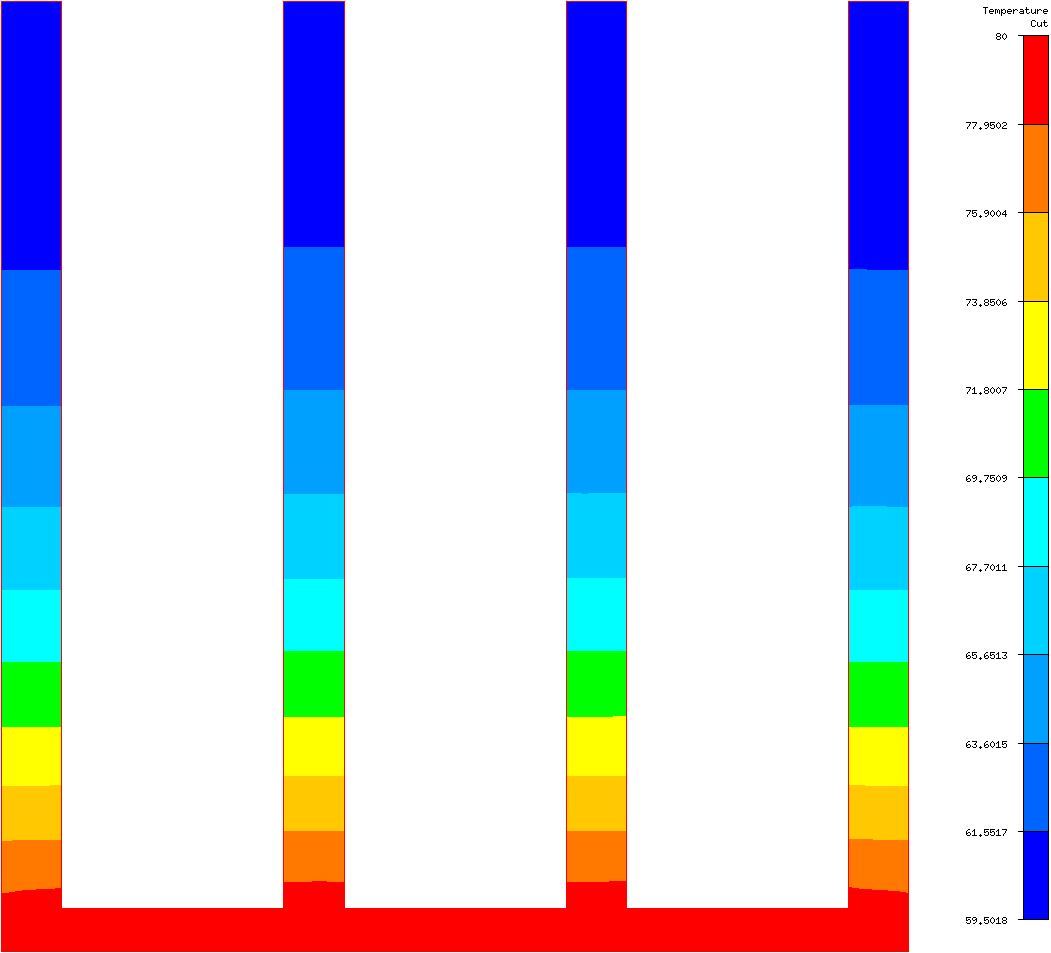
\includegraphics[width=0.7\textwidth]{../figures/heatsink4_h105_gmf005.png}
\caption{4 fins, \num{1.0} height}
\label{fig:mesh_temps_res_4_1}
\end{subfigure}
~
\begin{subfigure}[t] {0.23\textwidth}
\centering
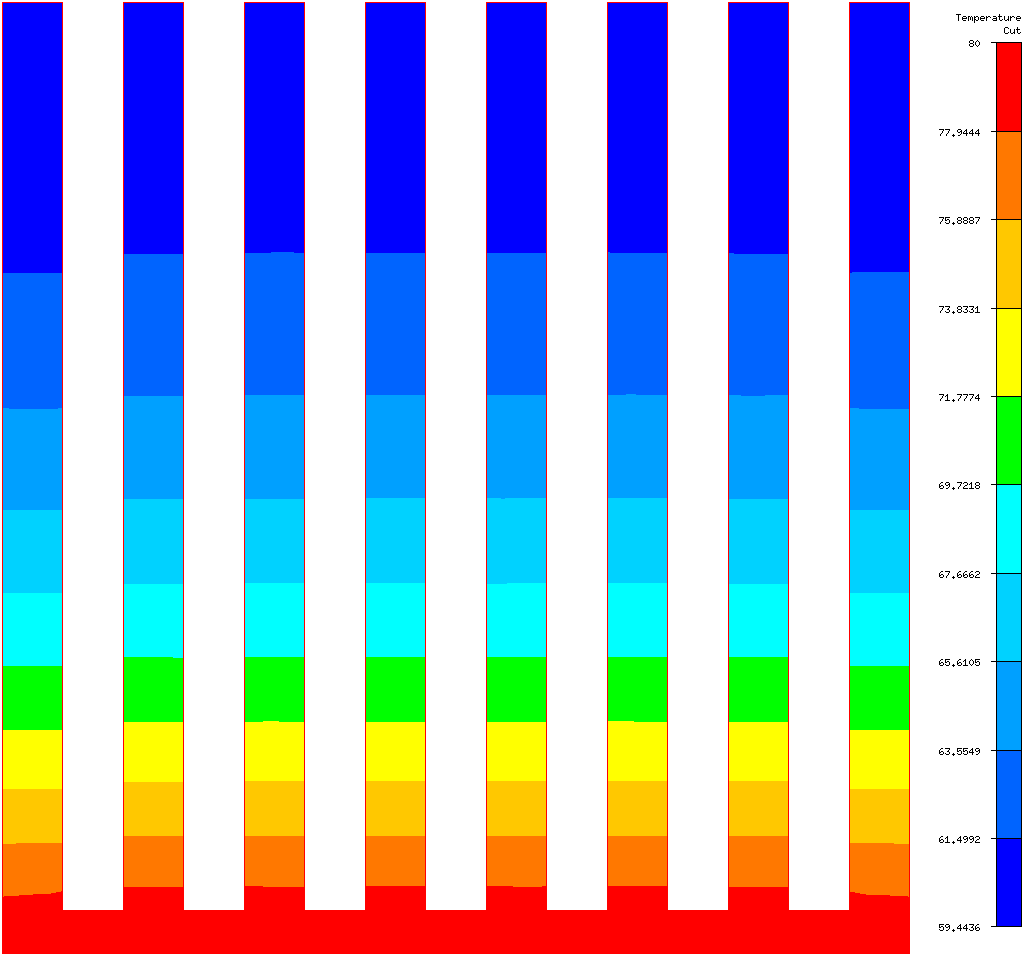
\includegraphics[width=0.7\textwidth]{../figures/heatsink8_h105_gmf005.png}
\caption{8 fins, \num{1.0} height}
\label{fig:mesh_temps_res_8_1}
\end{subfigure}
~
\begin{subfigure}[t] {0.23\textwidth}
\centering
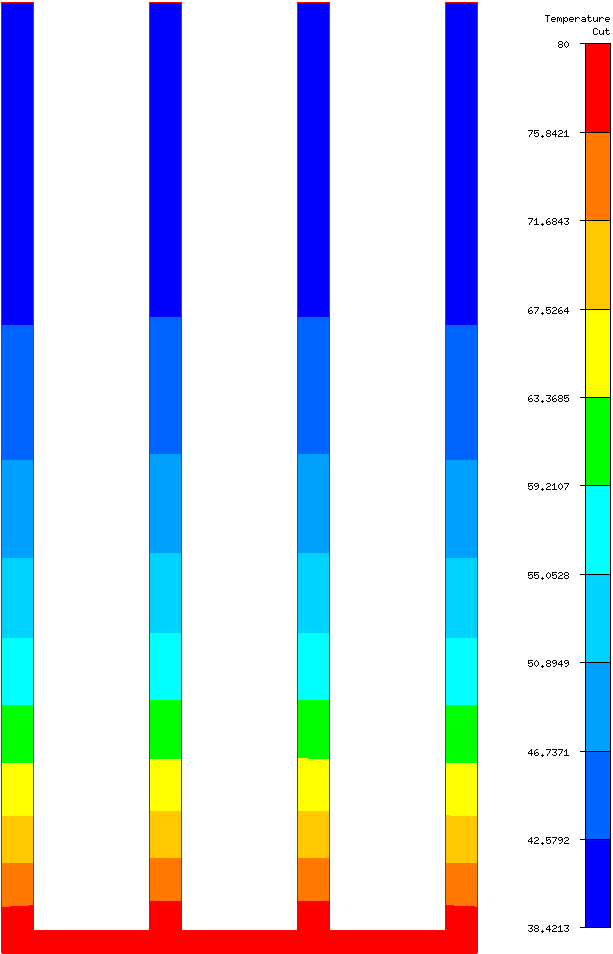
\includegraphics[width=0.7\textwidth]{../figures/heatsink4_h205_gmf005.png}
\caption{4 fins, \num{2.0} height}
\label{fig:mesh_temps_res_4_2}
\end{subfigure}
~
\begin{subfigure}[t] {0.23\textwidth}
\centering
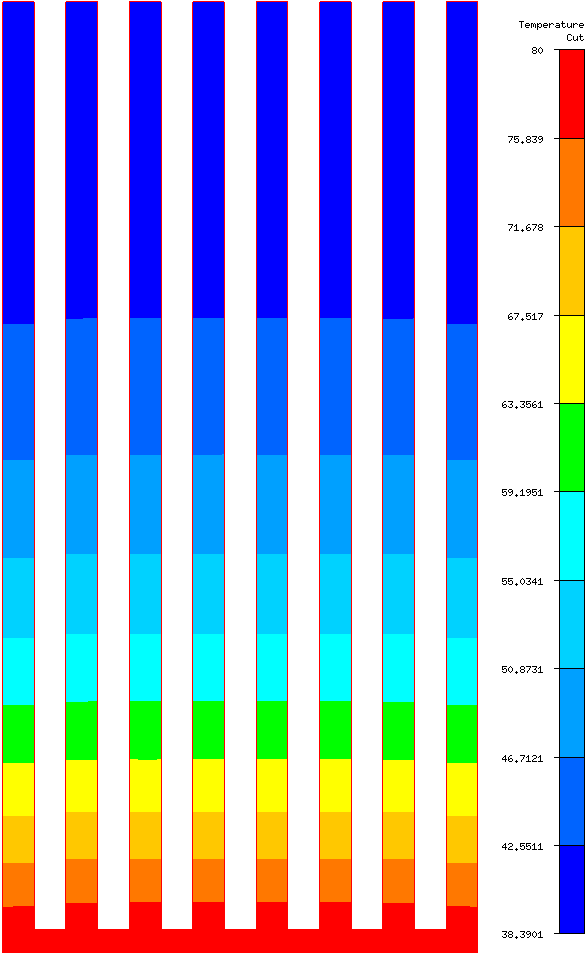
\includegraphics[width=0.7\textwidth]{../figures/heatsink8_h205_gmf005.png}
\caption{8 fins, \num{2.0} height}
\label{fig:mesh_temps_res_8_2}
\end{subfigure}
\caption{Temperatures in the middle of the heat sink for the different meshes.}
\label{fig:mesh_temps}
\end{figure}

In \cref{fig:mesh_temps} we can see the temperatures for the different meshes. The temperature ranges from about \SI{59}{\celsius} to \SI{80}{\celsius} for \cref{fig:mesh_temps_res_4_1} and \cref{fig:mesh_temps_res_8_1}, and from \SI{39}{\celsius} to \SI{80}{\celsius} for \cref{fig:mesh_temps_res_4_2} and \cref{fig:mesh_temps_res_8_2}. The Dirichlet boundary on the bottom works like a thermal reservoir, supplying as much heat as possible, so the temperature profiles along the fins are virtually identical between fins of the same height, regardless of the number of fins.

The total heat loss to the surrounding air is
\begin{equation}
\int_{\partial\Omega_R}\! \pdv{u}{n}\, \mathrm{d}{\gamma}.
\end{equation}
Since the heat flux in Robin boundary condition in \eqref{eq:heat_bvp} is proportional to the temperature difference, and we want to maximize the heat loss, a high temperature is preferred. The heat sink in \cref{fig:mesh_8_1} and \cref{fig:mesh_4_2} both have the same surface area and the same volume, however from figure \cref{fig:mesh_temps_res_8_1} we see that \cref{fig:mesh_8_1} generally have a higher temperature. The result is that \cref{fig:mesh_8_1} in total has a greater heat loss. It would appear that, given a certain amount of material, the heat sink should be designed with many short, thin fins, as opposed to fewer and higher fins. Because of this, tetrahedral elements may not be optimal for the type of geometries considered in this report. For instance, Comsol \cite{comsol_mesh_types} recommends to use brick or prism elements in cases where the geometry consists of thin layers.

\subsection{Assumptions and Physical Interpretation}
In our analysis we have made some assumptions and initial choices for the boundary conditions to make a somewhat simplified mathematical model. On the base of the heat sink base we enforced a constant Dirichlet boundary condition of \SI{80}{\celsius}, which is supposed to model an estimate of the temperature of a hot processor working at maximum capacity. By enforcing Dirichlet boundary condition we disallow the hypothetical processor to actually cool down, which is not necessarily a realistic assumption. When looking at a computer processor it would be natural to want to keep the temperature below some maximum threshold, and then look at how the heat sink would need to be engineered in order to have a sufficient heat loss, while the processor operates below this temperature. In that case some kind of Neumann boundary condition on the bottom would maybe be better suited in order to see such a cooling effect.

Another modeling choice made regarding the Robin conditions on the rest of the boundary is that the ambient temperature in the description of the boundary value problem \eqref{eq:heat_bvp} is also constant. This means that even in the tight spaces in between the fins the air temperature is constant. You could think of it as an average temperature on the boundary. One could maybe improve on this assumption by enforcing different ambient temperature on the outer boundary and the boundary in between the fins. Besides you would probably need a very powerful fan to transport the heat away to keep the ambient temperature at 20 degrees as assumed here.

If there were many more fins and they were a lot thinner and closer together it would be a good point to take into account the heat radiation from one fin to another. Also there would be challenges regarding the mesh. Using tetrahedron elements one could expect the elements to become very irregular. A solution could be to use brick prism elements, or alternatively a 2D mesh of the flat fins.

As stated in the introduction, copper is often used for heat exchanger because of its large thermal conductivity $k = \SI{401}{\watt\per\meter\per\kelvin}$, which is what used in this report. The heat conductivity is mainly material dependent, and therefore easy to handle. The heat transfer coefficient $h$, on the other hand, is a much more complicated matter. The effective $h$ will depend on the temperature range, air flow and geometry, among other factors. In this report we used $h \approx \SI{10}{\watt\per\meter\squared\per\kelvin}$, as estimated by \cite{heat_transfer_coeff} for a similar heat sink.
%% !TEX root = ../main/main.tex
\section{Conclusion and suggested next steps}
The aim of this report has been to explore how to use FEM to solve the heat equation on a heat sink. We wanted to investigate how to the temperature is distributed in heat sinks with different design options. Two of the design options had 4 fins, the other two had 8. Heights of 1.0 and 2.0 were tested for each option as well.

Some modeling choices was made in this report. Among them were the Dirichlet boundary condition on the base of the heat sink, the Robin boundary condition on the rest of the heat sink, and the constant temperature for the air surrounding the heat sink. These choices are possible to improve upon to make a better physical model. We would suggest to do some further studies on how the surrounding air temperature differentiates in between the fins as the average temperature is believed to be higher in these areas than on the outermost boundary. 

The results were found by solving the stationary heat equation on the geometry which was made in Gmsh for the purpose of this report. They would suggest that the design choice of having many fins has more effect than having fewer and higher fins.

Lastly in this report are some suggestions for next steps in this FEM analysis. As already mentioned the physical model could be improved upon. Also a more realistic case would be with much thinner and many more fins. This would create some challenges with the mesh because the tetrahedral elements could become irregular. One way of improving on this is to use brick prism elements, referring to \cite{comsol_mesh_types}. A way to work around this problem is to use 2D meshing for the fins. It is believed that this would be appropriate for very thin fins. Another next step would be to include the time derivative in the equation to study how the heat is dissipated in respect to time.

\nocite{*}
\bibliography{../bibl}
\bibliographystyle{plain}
\end{document}